\chapter{Разработка приложения} \label{chapt3}

Приложение логически делится на две большие части - серверную и клиентскую. В этой главе будут рассмотрены детали работы каждой из этих частей, а также сценарии их взаимодействия.

\section{Модули серверной части} \label{sect3_1}

Под серверной частью понимается совокупность скриптов на языке Python, отвечающая за следующие задачи:

\begin{itemize}
  \item Работа веб-сервера;
  \item Управление запуском и остановкой программ RTKRCV, STR2STR и CONVBIN пакета RTKLIB;
  \item Чтение и создание конфигурационных файлов для RTKRCV;
  \item Управление сохраненными на устройстве логами ГНСС данных.
\end{itemize}

\subsection{Низкоуровневая работа с RTKLIB. Класс RtkController} \label{subsect3_1_1}

В качестве основного средства извлечения контроля над программами пакета RTKLIB была выбрана библиотека Pexpect. Pexpect \cite{pexpect-docs} предоставляет возможность автоматизировать работу с интерактивными терминальными приложениями с помощью простой логики ожидания. Например, при запуске RTKRCV пользователь попадает в интерактивную консоль. Также, как и многие стандартные командные оболочки, к примеру \textbf{BASH}, перед ожиданием новой команды пользователя, RTKRCV выводит специальную последовательность символов - \textbf{rtkrcv>}. Pexpect предлагает следующую модель взаимодействия - отправить команду, а затем ждать контрольную строчку, показывающую что предыдущая команда обработана, а подконтрольное приложение готово принимать следующую. В приложении есть три класса, инкапсулирующие взаимодействие с программами RTKLIB:

\begin{itemize}
  \item \textbf{RtkController} работает с RTKRCV;
  \item \textbf{Str2StrController} работает c STR2STR;
  \item \textbf{ConvbinController} работает с CONVBIN.
\end{itemize}

Все они обладают свойством child, которому присваивается объект класса \textbf{Pexpect.spawn}. На листинге 3.1 - функция, запускающая RTKRCV.

\lstinputlisting[
  label={listings:RtkController_launch},
  caption={Метод launch класса RtkContoller},
  style={java}
]
{src/RtkController_launch.py}

В конструкторе класса \textbf{pexpect.spawn} происходит вызов программы RTKRCV с помощью команды из переменной \textbf{spawn\textunderscore command}. С помощью ключа «-o» указывается конфигурационный файл для загрузки. Следующий этап - проверка запуска на ошибку. Это происходит в функции \textbf{self.expectAnswer("spawn")}. Листинг 3.2 содержит функцию \textbf{expectAnswer()}.

\lstinputlisting[
  label={listings:RtkController_expectAnswer},
  caption={Метод expectAnswer класса RtkContoller},
  style={java}
]
{src/RtkController_expectAnswer.py}

Кроме возврата кода ошибки(или успеха) операции, вызывает метод expect класса \textbf{pexpect.spawn}. В качестве единственного параметра указан список строк. Метод \textbf{expect} читает стандартный вывод запущенной программы и ждет одну из этих строк. Под опцией \textbf{pexpect.EOF} понимается окончание работы программы. Таким образом, мы получаем представление о том, что же произошло с программой, запущенной с помощью \textbf{pexpect.spawn}.

Кроме того, чтобы запускать программу RTKRCV, мы должны также с ней взаимодействовать. Как только мы увидели, что вывод программы дошел до строки \textbf{rtkrcv>}, программа готова для дальнейшего взаимодействия. RTKRCV предлагает следующие команды консоли:

\begin{itemize}
  \item start. Запустить вычисления координат;
  \item stop. Остановить вычисления;
  \item load. Загрузить конфигурационный файл;
  \item status. Получить статус вычислений в виде текста;
  \item obs. Получить информацию о принимаемых сигналах спутников;
  \item shutdown. Завершить работу приложения.
\end{itemize}

Рассмотрим примеры работы с командами интерактивной консоли. Команды start, stop, load и shutdown работают по одной схеме: отправить команду, дождаться следующего вывода ключевой строки. На листинге 3.3 - функция, запускающая вычисления.

\lstinputlisting[
  label={listings:RtkController_start},
  caption={Метод start класса RtkContoller},
  style={java}
]
{src/RtkController_start.py}

Взаимодействие происходит по той же схеме - отправление команды, ожидание ответа. Если ответ не содержит слово \textbf{error} (RTKLIB всегда сообщает об ошибке в стандартный вывод), а приложение неожиданно не закончило свою работу, команда выполнена успешно.

Кроме таких команд, для которых требуется лишь подтверждение отсутствия ошибки, есть команды status и obs. Они возвращают статус в виде текста, который следует прочитать и извлечь из него полезную информацию. Информация, полученная с помощью команды status понадобится для отображения текущий координаты и качества решения. Obs возвращает таблицу, которая в том числе содержит signal to noise ratio(SNR), то есть уровни видимости спутников. Эта информация будет использоваться для графика на клиентской части приложения. Принцип работы в такой системе всегда один:

\begin{enumerate}
  \item Отправить команду исполняемому приложению;
  \item Получить ожидаемый ответ;
  \item Извлечь полезную информацию из ответа.
\end{enumerate}

На листинге 3.4 - функция, получающая статус RTKRCV.

\lstinputlisting[
  label={listings:RtkController_getStatus},
  caption={Метод getStatus класса RtkContoller},
  style={java}
]
{src/RtkController_getStatus.py}

Известно, что вывод команды status представляет собой набор строк, в которых параметр и его значение разделены двоеточиями. После получения подтверждения об отсутствии ошибки в выполнении, функция обращается к свойству \textbf{before}, представляющую весь вывод в виде одной строки. С помощью команды \textbf{split("\textbackslash r\textbackslash n")} можно разделить весь вывод на список отдельных строк, а затем обратиться к каждой из них с помощью цикла for. Если строка делится на две по символу «\textbf{:}», значит она содержит пару параметр-значение и подходит для добавление во внутреннюю переменную класса RtkController - status.

Работа с остальными программами RTKLIB - STR2STR и CONVBIN происходит ровно таким же образом, за тем исключением, что они не имеют интерактивной консоли и автоматизация ограничивается запуском с правильными ключами и параметрами, а также чтением результатов работы из стандартного вывода.

\subsection{Работа с конфигурационными файлами. Класс ConfigManager} \label{subsect3_1_2}

Как уже упоминалось, RTKRCV использует конфигурационные файлы для хранения и изменения многочисленных настроек. Приложение должно уметь читать эти файлы, для того чтобы правильно отображать эти настройки в клиентской части, а также перезаписывать измененные в браузере значения. Для этого создан класс ConfigManager. Он служит для того, чтобы:

\begin{itemize}
  \item Возвращать список доступных конфигурационных файлов;
  \item Читать файлы и возвращать словарь настроек;
  \item Создавать файл из словаря настроек;
  \item Сбросить файл до значения по умолчанию;
  \item Удалить файл.
\end{itemize}

Для работы этого класса используется вспомогательный класс \textbf{Config}, который принимает путь к конфигурационному файлу как единственный параметр конструктора и прочитав файл, создает словарь значений. Рассмотрим пример конфигурационного файла RTKRCV изображен на листинге 3.5.

\lstinputlisting[
  label={listings:RTKLIB_conf_file},
  caption={Отрывок конфигурационного файла RTKRCV},
  style={java}
]
{src/rtkrcv_conf_snippet.conf}

У некоторых строк есть комментарии. Эти комментарии, отделенные одним символом \textbf{\#}, показывают возможные варианты значений параметра. Комментарии отделенные \textbf{\#\#}, используются для подписей параметров в форме на веб-странице. При чтении файла, каждая строка читается и собирается в словарь с четырьмя полями(пример - на листинге 3.6).

\lstinputlisting[
  label={listings:conf_parameter},
  caption={Представление параметра конфигурационного файла в памяти},
  style={java}
]
{src/conf_parameter.py}

Этот класс используется более общим классом RTKLIB, речь о котором пойдет в следующей части.

\subsection{Высокоуровневая работа с RTKLIB. Класс RTKLIB} \label{subsect3_1_4}

Класс RTKLIB берет на себя почти все функции, связанные с управлением программами пакета RTKLIB. Через методы и свойства этого класса сервер работает с программами, логами и конфигурационными файлами.

Рассмотрим основные функции класса RTKLIB:

\begin{itemize}
  \item Переключение между режимами ровера и базы;
  \item Запуск и остановка ровера и базы;
  \item Чтение и запись настроек ровера и базы;
  \item Конвертация логов данных в другой формат;
  \item Сохранение и загрузка режима работы;
  \item Трансляция координат и уровней спутников на front-end.
\end{itemize}

Основной задачей этого класса является инкапсуляция всех нюансов работы с отдельными частями RTKLIB. Например этот класс берет на себя обработку ошибок в работе классов более низкого уровня.

Одни из самых главных понятий, определенных в классе RTKLIB - состояния ровера и базы. Дело в том, что RTKLIB сам по себе не предполагает таких ролей. Есть RTKRCV, занимающийся расчетом координат с помощью совмещения показаний двух приемников. Также есть STR2STR, который позволяет перенаправлять потоки данных ГНСС приемников. Однако, STR2STR - единственная программа пакета, которая способна выдавать данные в легковесном формате RTCM3. Поэтому в классе RTKLIB запуск режима ровера равносилен запуску RTKRCV с помощью класса RtkController, а запуск режима базы - запуску STR2STR с помощью Str2StrController.

Функции записи настроек - writeConfigRover или writeConfigBase передают управление различным классам более низкого уровня - ConfigManager и Str2StrController. Причина этого кроется в том, что STR2STR не нуждается в конфигурационных файлах. Все настройки передаются через параметры запуска приложения. Таким образом, в случае с ровером нужна перезапись файла на диске, а в случае с базой - достаточно изменить свойства класса Str2StrController.

Кроме передачи управления другим классам у RTKLIB есть своя уникальная функциональность. Например, с помощью функций \textbf{saveState} и \textbf{loadState}, класс записывает и загружает все настройки. Если настройки RTKRCV сохраняются в файлы, то остальные настройки, такие как режим базы или ровера, а также настройки базы, надо хранить отдельно. При выполнении любой операции, затрагивающей изменения настроек вызывается \textbf{saveState}. Внутри функции информация собирается в словарь, который переводится в JSON формат с помощью стандартного модуля \textbf{json}. При загрузке, которая проходит при запуске приложения этот файл считывается, JSON декодируется обратно в Python словарь и запускаются соответствующие методы класса RTKLIB, чтобы продолжить работу с том же состоянии. Это очень полезно, если приложение запускается при загрузке операционной системы. Таким образом, можно продолжать работу в том же режиме после включения устройства без необходимости залезать в настройки.

Еще одна важная функция, которую на себя берет класс RTKLIB - трансляция координат и уровней спутников в браузер посредством веб-сокетов. При старте в режиме ровера, создаются и запускаются два новых потока: \textbf{satellite\_ thread} и \textbf{coordinate\_ thread}. Эти потоки выполняют методы класса RTKLIB \textbf{broadcastCoordinates} и \textbf{broadcastSatellites}(листинг 3.7).

\lstinputlisting[
  label={listings:RTKLIB_broadcastSatellites},
  caption={Метод broadcastSatellites класса RTKLIB},
  style={java}
]
{src/RTKLIB_broadcastSatellites.py}

Эта функция заключается в бесконечном цикле, постоянно считывающем статус из RTKRCV и отправлюящем его в браузер с помощью объекта \textbf{socketio}. В случае остановки в режиме ровера, свойство \textbf{server\_ not\_ interrupted} становится \textbf{False} и поток заканчивает свое выполнение.

\subsection{Запуск главной программы и сервера. Модуль server.py} \label{subsect3_1_5}

Главным файлом в проекте является \textbf{server.py}. Основными функциями модуля являются:

\begin{itemize}
  \item Создание и запуск сервера;
  \item Инициализация объекта класса RTKLIB для работы с RTK функциями;
  \item Создание обработчиков HTTP запросов;
  \item Создание обработчиков WebSocket событий.
\end{itemize}

Листинг 3.8 - инициализация сервера.

\lstinputlisting[
  label={listings:server_init},
  caption={Инициализация сервера Flask},
  style={java}
]
{src/server_init.py}

Фрэймворк Flask имеет модульную архитектуру, поэтому WebSocket функциональность реализована в расширении Flask-socketio. Для того чтобы подключить данное расширение, следует передать объект класса Flask в конструктор класса SocketIO. После этого переменная \textbf{app} имеет возможность обрабатывать события, связанные с веб-сокетами. Это стандартный способ добавления Flask расширений в сервер.

Так как предложение имеет лишь одну страницу, а вся навигация происходит строго в браузере, то на сервере зарегистрированы лишь два обработчика HTTP запросов - для самой страницы(лист. 3.9) и для загрузки логов(лист. 3.10).

\lstinputlisting[
  label={listings:server_http_handler},
  caption={Обработчик HTTP запроса в Flask приложении},
  style={java}
]
{src/server_http_handler.py}

\lstinputlisting[
  label={listings:file_download_http_server},
  caption={Скачивание файла в Flask приложении},
  style={java}
]
{src/file_download_http_server.py}

Большая часть данного модуля - регистрация обработчиков событий, связанных с веб-сокетами. Синтаксис у них такой же. Например, обработка события запуск режима ровера описана на листинге 3.11.

\lstinputlisting[
  label={listings:server_websocket_handler},
  caption={Обработчик WebSocket события в Flask приложении},
  style={java}
]
{src/server_websocket_handler.py}

Следует обратить внимание на особенность синтаксиса в этих примерах. Декораторы используются для привязки нижеописанных функций к событиям, переданным в качестве параметров декоратору.

Главный цикл состоит из одного действия(лист. 3.12). В нем запускается сервер и обрабатывается исключение KeyboardInterrupt(нажатие CTRL+C), корректно завершая все потоки.

\lstinputlisting[
  label={listings:main_loop},
  caption={Главный цикл Flask приложения},
  style={java}
]
{src/main_loop.py}

\section{Веб-страница и модули клиентской части} \label{sect3_2}

Под клиентской частью понимается веб-страница и совокупность скриптов на языке Javascript, отвечающие за следующие задачи:

\begin{itemize}
  \item Отображение статуса RTKLIB;
  \item Отображение форм настройки RTKLIB;
  \item Отображение списка логов данных.
\end{itemize}

\subsection{Основа клиентской части - HTML страница} \label{subsect3_2_1}

Весь интерфейс приложения строится вокруг одной HTML страницы. Все элементы на странице выбраны из стандартных элементов UI фрэймворка jQuery Mobile. Общая структура документа - несколько \textbf{div} элементов со свойством \textbf{data-role} выставленным на значение \textbf{"page"}(лист. 3.13). Это дает возможность перемещаться между различными экранами без необходимости перезагрузки страницы, или обращения к серверу, как к таковому.

\lstinputlisting[
  label={listings:jqm_element_example},
  caption={Создание элемента-страницы в jQuery Mobile},
  style={java}
]
{src/jqm_element_example.html}

Кроме основных элементов, в HTML файле создаются диалоговые окна. Они остаются невидимыми для пользователя до тех пор, пока не приходит нужный момент. Пример всплывающего окна, появляющегося при потере связи с сервером - на листинге 3.14).

\lstinputlisting[
  label={listings:popup_window},
  caption={Создание всплывающего окна в jQuery Mobile},
  style={java}
]
{src/popup_window.html}

Сама по себе страница - лишь скелет для запуска клиентских скриптов. Все основные изменения внутри страницы и приложения, такие как обновление информации на графике или создание и отправка данных формы происходят с помощью Javascript.

\subsection{Инициализация клиента. Модуль main.js} \label{subsect3_2_2}

Модуль \textbf{main.js} важен как место инициализации объекта, олицетворяющего соединения с сервером(лист. 3.15). Он используется для связи с сервером. С помощью переменной \textbf{socket} создаются обработчики различных WebSocket сообщений \cite{socketio-docs}.

\lstinputlisting[
  label={listings:websocket_object},
  caption={Создание объекта для приема WebSocket сообщений},
  style={java}
]
{src/websocket_object.js}

Рассмотрим, как происходит обработка приходящих сообщений. Для того, чтобы, например, отображать координаты, надо обрабатывать сообщения с заголовком \textbf{"coordinate broadcast"}(лист. 3.16).

\lstinputlisting[
  label={listings:coordinate_broadcast},
  caption={Обработка сообщения \textbf{"coordinate broadcast"} на стороне клиента},
  style={java}
]
{src/coordinate_broadcast.js}

Извлеченные данные, в переменной msg передаются в функцию \textbf{updateCoordinateGrid}, выставляющую значения пришедших координат в нужные элементы на странице. Со стороны сервера эти сообщения отправляет поток, созданный из функции \textbf{broadcastCoordinates}, описанный в главе 3.1.3.

\subsection{Обработка взаимодействия пользователя с элементами страницы. Модуль handlers.js} \label{subsect3_2_3}

Модуль handlers.js в первую очередь предназначен для «оживления» элементов страницы. В нем регистрируются обработчики большинства событий связанных с интерфейсом приложения. Примером могут служить такие взаимодействия, как отправление команды запуска ровера и по нажатию кнопки или изменение отображаемого конфигурационного файла при изменении значения селектора(лист. 3.17).

\lstinputlisting[
  label={listings:start_handler},
  caption={Регистрация обработчика нажатия на кнопку start},
  style={java}
]
{src/start_handler.js}

Кнопка \textbf{start} при нажатии отправляет сообщение \textbf{«start rover»} или \textbf{«start base»}, в зависимости от режима и становится невидимой, уступив место кнопке \textbf{stop}.

Также, подобные события можно привязать к менее очевидным элементам интерфейса. Например, каждый раз, при переходе во вкладку \textbf{Logs}, браузер отправляет запрос о текущем количестве логов и свободном пространстве на устройстве(лист. 3.18).

\lstinputlisting[
  label={listings:logs_tab_handler},
  caption={Обработка перехода на вкладку \textbf{Logs}},
  style={java}
]
{src/logs_tab_handler.js}

\subsection{График уровней приема спутников. Модуль graph.js} \label{subsect3_2_3}

Модуль \textbf{graph.js} содержит функции, отвечающие за работу с графиком:

\begin{itemize}
  \item Инициализация графика;
  \item Перерисовка при изменении размера окна браузера;
  \item Обновление значений на графике.
\end{itemize}

График написан с помощью библиотеки \textbf{D3.js}. Вся анимация создается в специальном HTML тэге - <svg>(лист. 3.19).

\lstinputlisting[
  label={listings:graph_golder},
  caption={Инициализация \textbf{svg} элемента для создания графика},
  style={java}
]
{src/graph_holder.js}

Результат представляет собой гистограмму, столбцы которой отражают различные спутники, а их высота показывает качество приема данного спутника. Качество выражается значением величины «отношение сигнал/шум»(\textbf{signal to noise ratio} или \textbf{SNR}), полученным из RTKLIB. На графике помещается не больше десяти значений с лучшим приемом. Если ровер получает поправки от базы, то на графике также отображаются значения SNR тех же спутников для базы(рис. 3.1).

\begin{figure}[ht]
  \center
  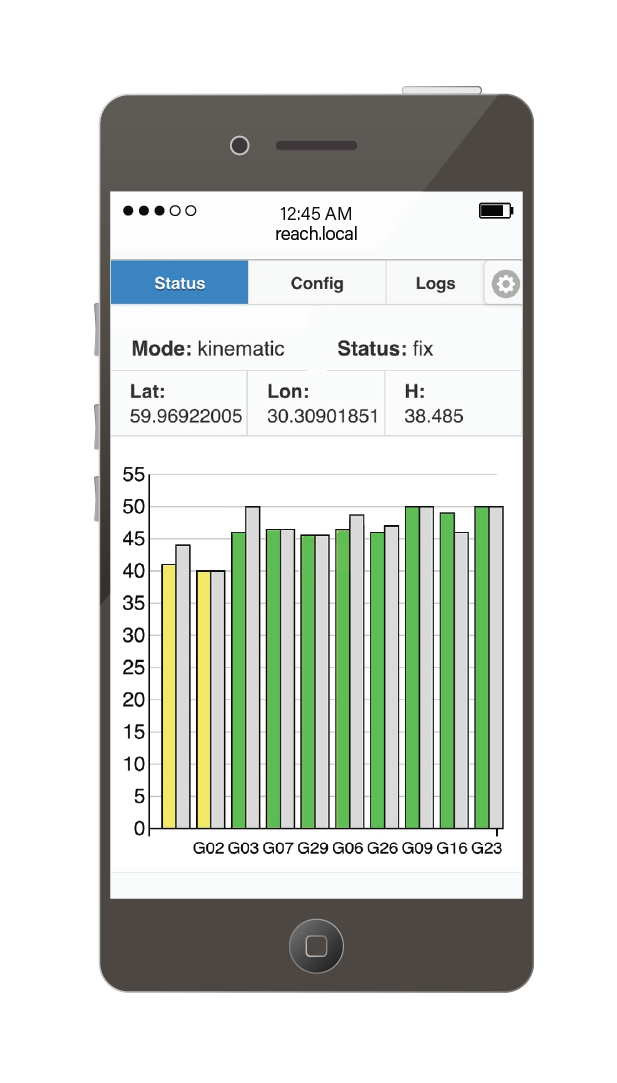
\includegraphics [scale=0.7] {SNR_chart}
  \caption{График уровней приема спутников}
  \label{img:latex}
\end{figure}

\subsection{Создание и чтение форм конфигурации. Модуль config.js} \label{subsect3_2_3}

Модуль \textbf{config.js} отвечает за работу с формами. Конфигурационные файлы RTKRCV, так же как и настройки STR2STR, которые задаются с помощью параметров запуска, имеют особенный синтаксис, особенно при задании входящих и исходящих потоков данных. Например, для того чтобы настроить RTKRCV на вывод координат через последовательный интерфейс, нужно выставить значения трех переменных, как на листинге 3.20.

\lstinputlisting[
  label={listings:rtkrcv},
  caption={Настройка вывода координат из RTKRCV},
  style={java}
]
{src/rtkrcv.conf}

Задача модуля \textbf{config.js} отобразить эти самые настройки в удобном для чтения и изменения виде. При запуске с такими настройками RTKRCV обратится к \textbf{/dev/ttyMFD2} с настройкой скорости передачи данных 230400 бод. Пользователю неудобно работать с такой строкой и поэтому форма с настройками во вкладке \textbf{Config} превратит данную строку в раскрытую форму. Третья опция изменяет формат вывода на \textbf{llh}, или широта, долгота, высота и представлена отдельным селектором, следующей опцией. Результат отображения представлен на рисунке 3.2.

\begin{figure}[ht]
  \center
  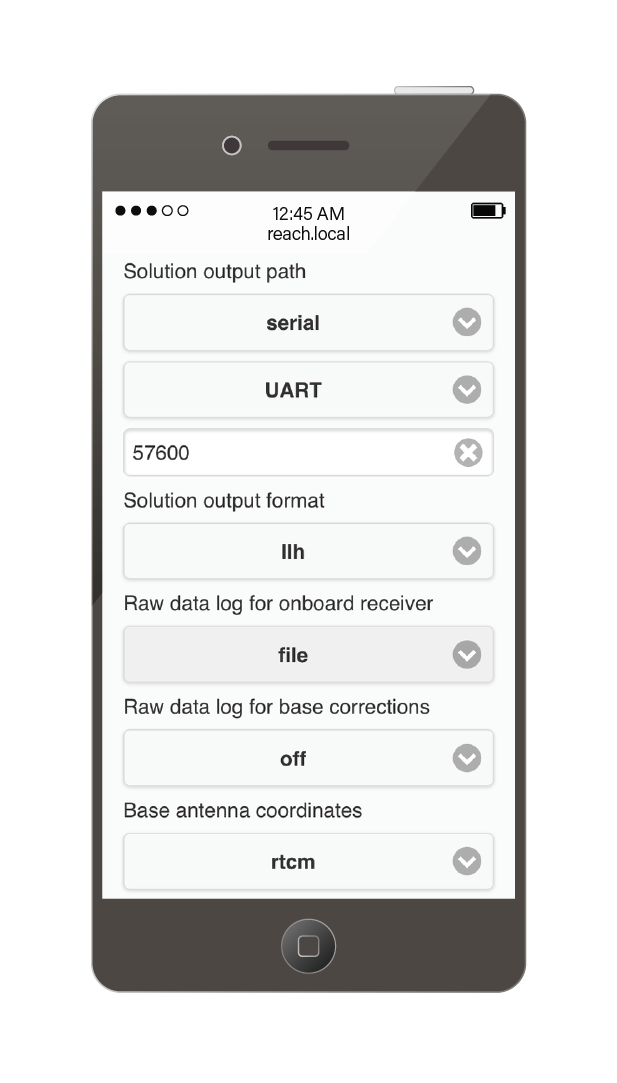
\includegraphics [scale=0.7] {Serial_form}
  \caption{Настройка вывода координат в формате llh в последовательный порт}
  \label{img:latex}
\end{figure}

Также, \textbf{config.js} выполняет обратную функцию - при изменении данных, нужно собрать данные формы в совместимые с RTKLIB строки. Для этого используются скрытые от пользователя строки, которые обновляются при любом изменении данных в форме.

\clearpage

\section{Сценарии взаимодействия сервера и клиента} \label{sect3_3}

В данной главе рассмотрены основные сценарии взаимодействия пользователя, браузера, сервера и управляемых ими классов. На рисунке 3.3 изображена диаграмма обработки запроса веб-страницы приложения.

\begin{figure}[ht]
  \center
  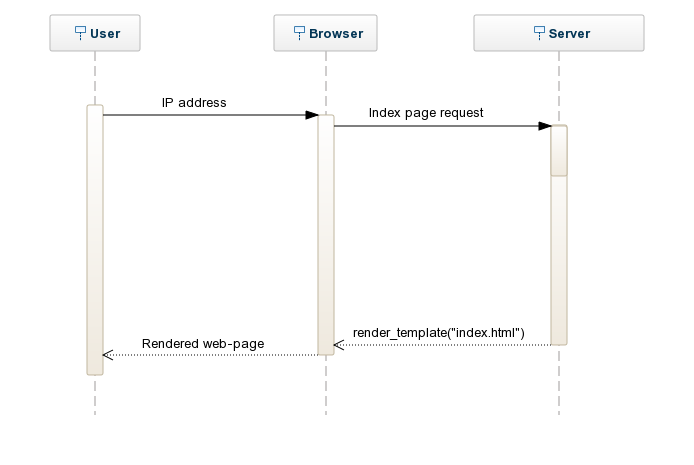
\includegraphics [scale=0.4] {uml_index_request}
  \caption{Обработка запроса веб-страницы}
  \label{img:latex}
\end{figure}

\clearpage

После загрузки страницы все взаимодействия происходят с помощью WebSockets. Например, при переходе во вкладку Config, происходит запрос текущего конфигурационного файла RTKRCV для отображения формы. Более подробно этот процесс рассмотрен на рисунке 3.4.

\begin{figure}[ht]
  \center
  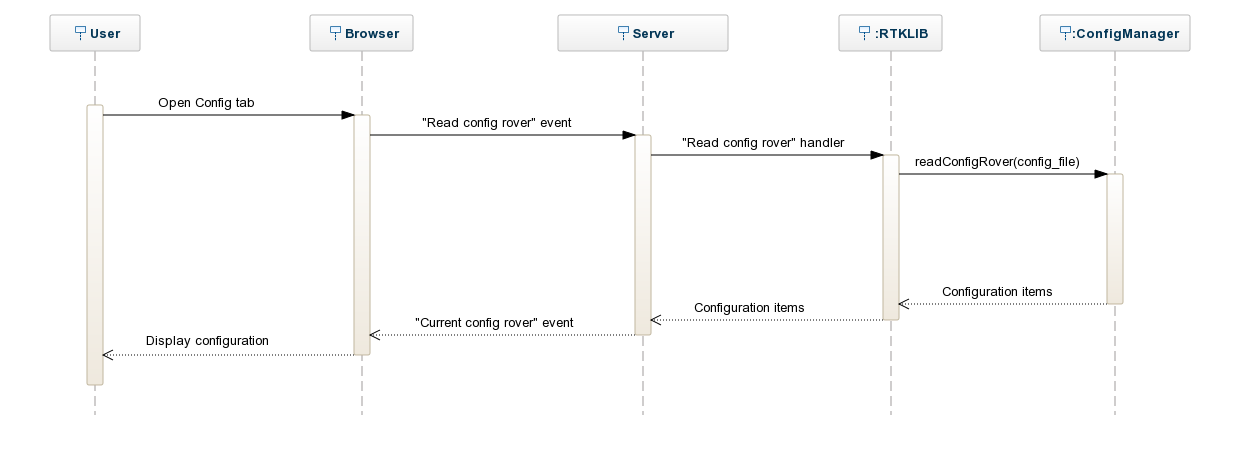
\includegraphics [scale=0.3] {uml_config_read}
  \caption{Чтение конфигурационного файла для отображения на веб-странице}
  \label{img:latex}
\end{figure}

\clearpage

При взаимодействии с элементами страницы также могут происходить события, отправляющие команды или запросы на сервер. Так, на рисунке 3.5 изображен процесс старта RTKRCV.

\begin{figure}[ht]
  \center
  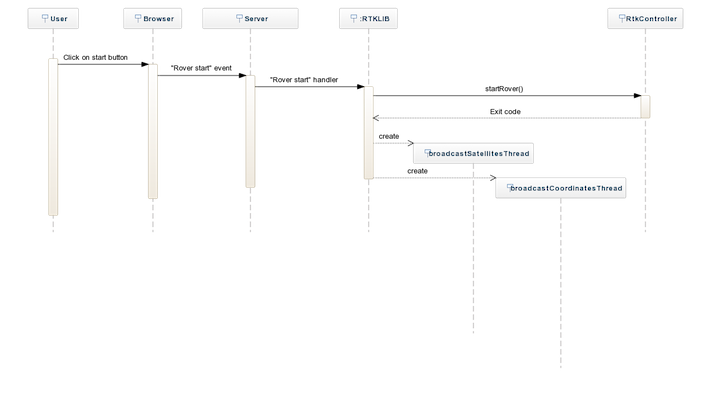
\includegraphics [scale=0.5] {uml_rover_start_copy}
  \caption{Запуск RTKRCV}
  \label{img:latex}
\end{figure}

\clearpage

Другим примером такого взаимодействия является сохранение и загрузка конфигурационного файла RTKRCV(рис. 3.6).

\begin{figure}[ht]
  \center
  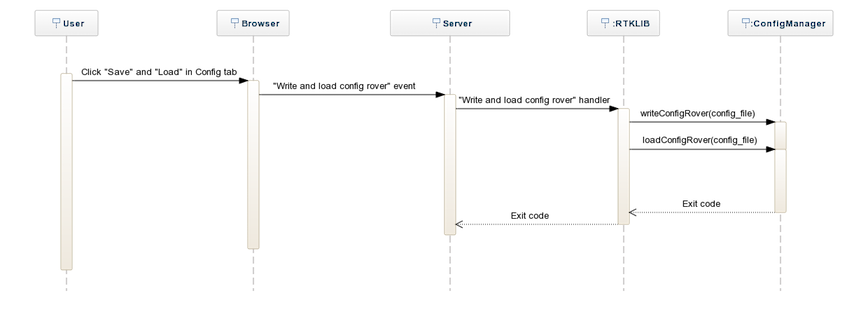
\includegraphics [scale=0.4] {uml_write_config_copy}
  \caption{Сохранение и загрузка конфигурационного файла}
  \label{img:latex}
\end{figure}

\clearpage

При загрузке логов, заранее неизвестно, переведен файл в формат RINEX или нет. Поэтому, вместо прямых ссылок на файлы, клиент отправляет запрос, по которому сервер генерирует ссылку на готовый лог, в зависимости от доступного формата файла(рис. 3.7).

\begin{figure}[ht]
  \center
  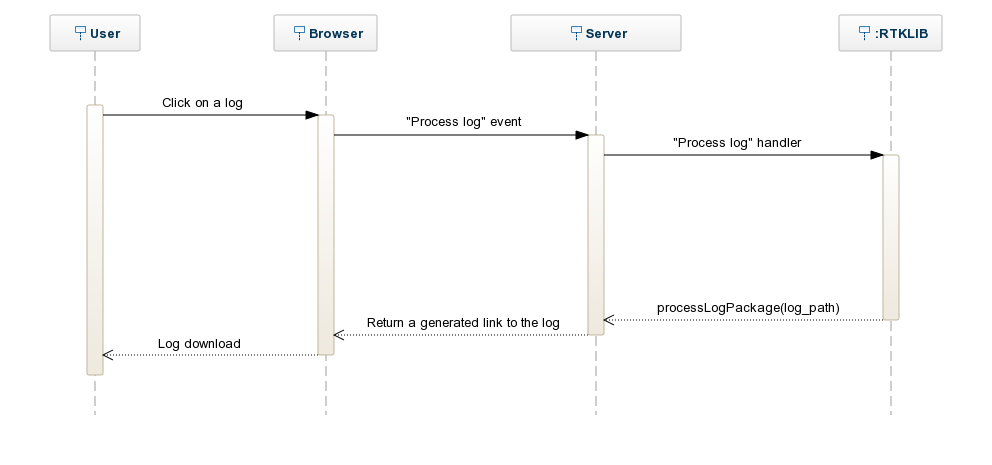
\includegraphics [scale=0.3] {uml_log_download}
  \caption{Загрузка логов}
  \label{img:latex}
\end{figure}

\clearpage

\section{Результаты разработки} \label{sect3_4}

В результате было разработано приложение, удовлетворяющее вышеназванным требованиям. На рисунке 3.8 приведено дерево конечного проекта, включающего все модули.

\begin{figure}[ht]
  \center
  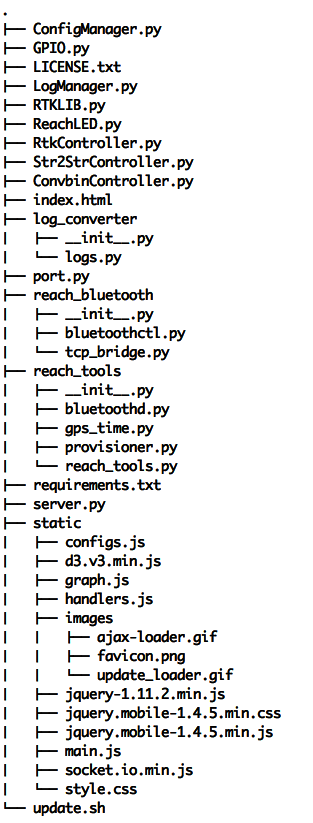
\includegraphics [scale=0.4] {project_tree}
  \caption{Дерево разработанного проекта}
  \label{img:latex}
\end{figure}

Были разработаны классы, инкапсулирующие работу с RTKLIB:

\begin{itemize}
  \item RtkController - работа с RTKRCV;
  \item Str2StrController - работа с STR2STR;
  \item ConvbinController - работа с CONVBIN;
  \item ConfigManager - управление конфигурационными файлами;
  \item LogManager - управление логами;
  \item RTKLIB - инкапсуляция работы всех вышеперечисленных файлов.
\end{itemize}

Модуль server.py, отвечающий за обработку HTTP и WebSocket запросов.

Веб-страница index.html, являющаяся основой одностраничного приложения. Для ее работы используются Javascript модули:

\begin{itemize}
  \item main.js - создание обработчика WebSocket сообщений, общая инициализация;
  \item config.js - работа с формами во вкладке Config;
  \item handlers.js - работа с интерфейсом страницы;
  \item graph.js - работа с графиком.
\end{itemize}

Кроме этого, в проекте присутствуют служебные модули, отвечающие за работу приложения на Emlid Reach:

\begin{itemize}
  \item reach\_tools.py - набор утилит, в числе которых определение свободного места, отведенного под логи, а также установка системного времени по GPS;
  \item reach\_bluetooth - инициализация Bluetooth на устройстве и создание TCP - Bluetooth моста, для передачи ГНСС данных через Bluetooth.
\end{itemize}

На группе рисунков 3.9 изображены все вкладки приложения.

\begin{figure}
  \label{img:latex}
  \begin{subfigure}{\linewidth}
    \center
    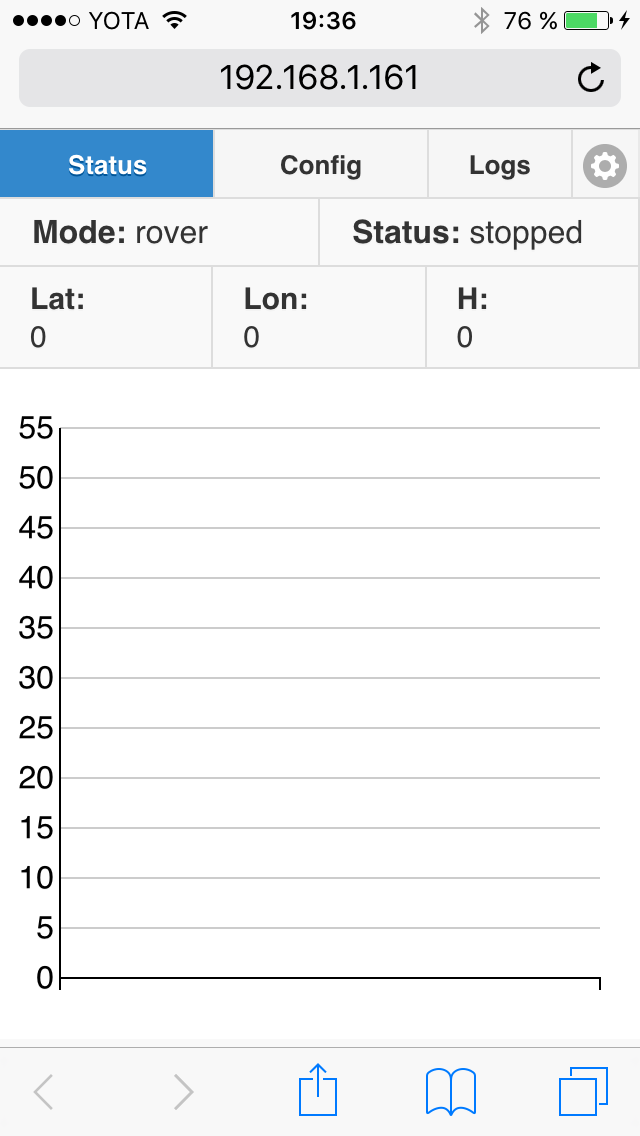
\includegraphics[width=.35\linewidth]{ui_testing_status_tab}
    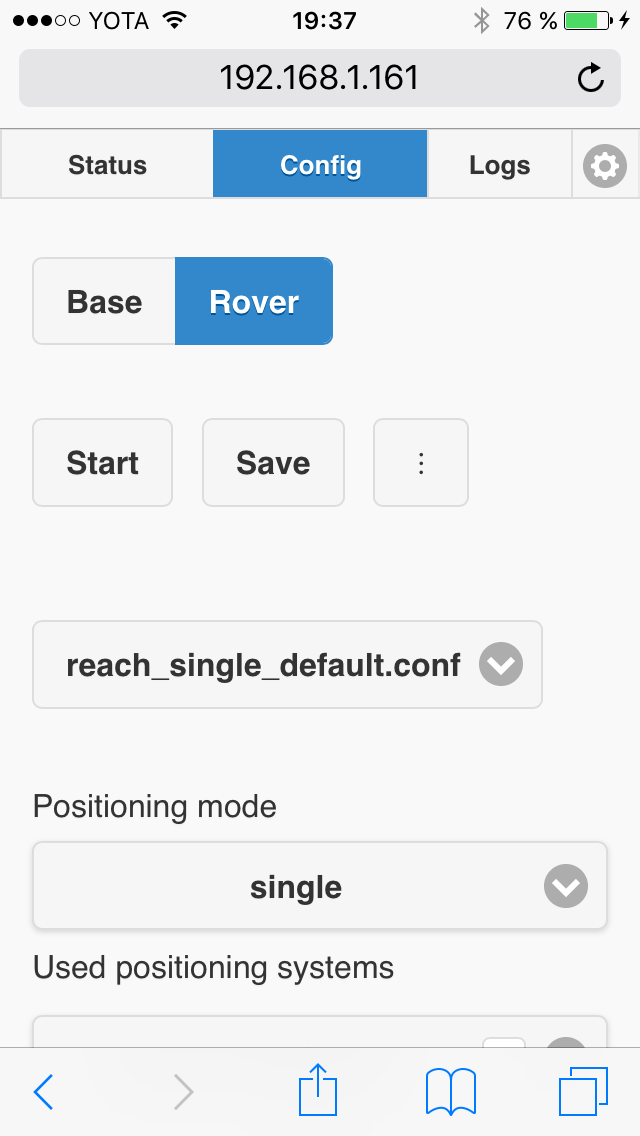
\includegraphics[width=.35\linewidth]{ui_testing_config_tab}
    \caption{Status и Config}
  \end{subfigure}\par\medskip
  \begin{subfigure}{\linewidth}
    \center
    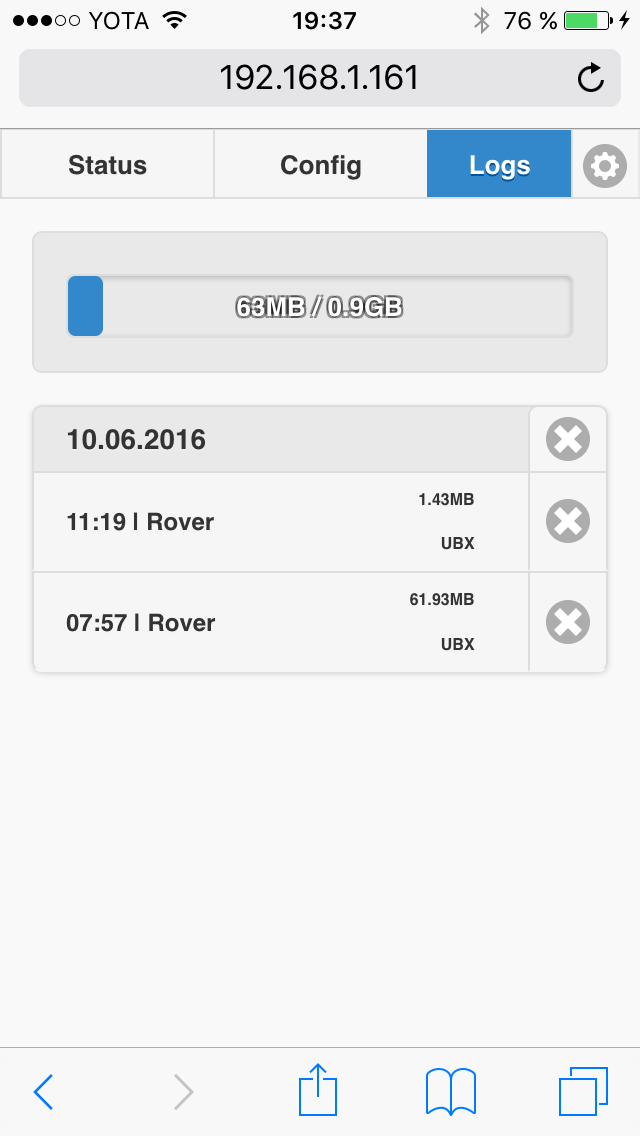
\includegraphics[width=.35\linewidth]{ui_testing_logs_tab}
    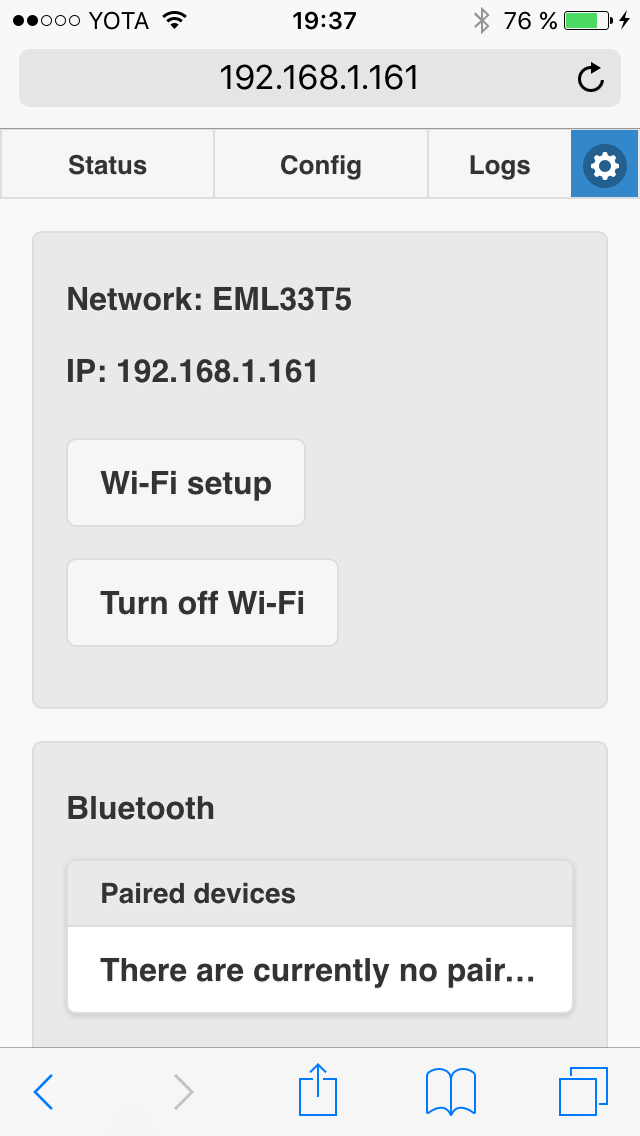
\includegraphics[width=.35\linewidth]{ui_testing_settings_tab}
    \caption{Logs и Settings}
  \end{subfigure}\par\medskip
  \caption{Вкладки приложения в браузере смартфона}
\end{figure}